\section{Auswertung}
\label{sec:Auswertung}

        \subsection{Invertierender Linearverstärker}

            \subsubsection{Messwerte}

                Es werden vier Messreihen mit unterschiedlichen Widerstandsverhältnissen und 
                Eingangsspannungen, welche in Tabelle \ref{tab:inv1} zu finden sind, vorgenommen.
                Die Phasen- und Ausgangsspannungswerte mit zugehöriger Frequenz für die jeweiligen 
                Messreihen sind in den Tabellen \ref{tab:inv2} bis \ref{tab:inv5} eingetragen.

                \begin{table}
                    \centering
                    \caption{Eingangsspannungen und Widerstandsverhältnisse der vier Messreihen
                    für den invertierenden Linearverstärker.}
                    \label{tab:inv1}
                    \begin{tabular}{c r r r r}
                        \toprule
                            Messreihe & $U_e$/mV & $R_1$/k$\symup{\Omega}$ & $R_N$/k$\symup{\Omega}$ & $\frac{R_N}{R_1}$\\
                        \midrule
                           1 & 110 & 1,00 & 10,00 & 10,00\\
                           2 & 310 & 1,00 & 33,10 & 33,10\\
                           3 & 310 & 10,00 & 33,10 & 3,31\\
                           4 & 310 & 33,10 & 98,00 & 2,96\\
                        \bottomrule
                    \end{tabular}
                \end{table}

                \begin{table}
                    \centering
                    \caption{Erhobene Daten der ersten Messreihe für den invertierenden Linearverstärker
                    mit Widerstandsverhältnis 10 und Eingangsspannung 110\,mV.}
                    \label{tab:inv2}
                    \begin{tabular}{c c c c}
                        \toprule
                            Frequenz/kHz &  Phase/°& Ausgangsspannung/V \\
                        \midrule
                             0,99 & 177,0 & 0,87\\
                             2,00 & 178,7 & 0,88\\ 
                             2,99 & 178,0 & 0,88\\ 
                             4,00 & 180,6 & 0,88\\
                             5,00 & 179,6 & 0,88\\
                             5,99 & 177,6 & 0,88\\
                             6,99 & 179,3 & 0,88\\
                             7,99 & 177,8 & 0,88\\
                             8,99 & 179,0 & 0,88\\
                            10,02 & 177,0 & 0,88\\
                            10,99 & 175,0 & 0,88\\
                            12,01 & 177,0 & 0,87\\
                            12,99 & 173,0 & 0,87\\
                            15,99 & 173,0 & 0,87\\
                            19,97 & 171,0 & 0,87\\
                            50,00 & 156,0 & 0,81\\
                            60,10 & 154,0 & 0,80\\
                            79,60 & 142,0 & 0,73\\
                            89,90 & 140,0 & 0,70\\
                           151,00 & 120,0 & 0,53\\
                           202,00 & 110,0 & 0,44\\
                           298,00 &  90,0 & 0,31\\
                           400,00 & 100,0 & 0,24\\
                           500,00 &  90,0 & 0,20\\
                           600,00 &  70,0 & 0,17\\
                           690,00 &  80,0 & 0,15\\
                           780,00 &  70,0 & 0,13\\
                           890,00 &  50,0 & 0,12\\
                        \bottomrule
                    \end{tabular}
                \end{table}    

                \begin{table}
                    \centering
                    \caption{Erhobene Daten der zweiten Messreihe für den invertierenden Linearverstärker 
                    mit Widerstandsverhältnis 33,1 und Eingangsspannung 310\,mV.}
                    \label{tab:inv3}
                    \begin{tabular}{c c c c}
                        \toprule
                            Frequenz/kHz & Phase/° & Ausgangsspannung/V \\
                        \midrule
                            1,00 & 175,1 & 9,77\\
                            2,00 & 178,9 & 9,77\\ 
                            3,00 & 178,3 & 9,73\\ 
                            4,00 & 173,6 & 9,73\\
                            5,00 & 170,9 & 9,69\\
                            5,99 & 167,7 & 9,61\\
                            6,99 & 166,0 & 9,57\\
                            7,99 & 163,5 & 9,45\\
                            8,99 & 154,0 & 9,33\\
                           20,03 & 111,0 & 6,03\\
                           30,00 &  87,0 & 3,78\\
                           40,10 &  91,0 & 2,97\\
                           50,20 &  90,0 & 2,65\\
                           60,10 &  95,0 & 2,33\\
                           79,60 &  89,0 & 1,85\\
                          100,00 &  90,0 & 1,53\\
                          120,00 &  90,0 & 1,33\\
                          198,00 &  80,0 & 0,84\\
                          250,00 &  90,0 & 0,72\\
                          300,00 &  60,0 & 0,60\\
                          500,00 &  70,0 & 0,36\\
                        \bottomrule
                    \end{tabular}
                \end{table}            

                \begin{table}
                    \centering
                    \caption{Erhobene Daten der dritten Messreihe  für den invertierenden Linearverstärker 
                    mit Widerstandsverhältnis 3,31 und Eingangsspannung 310\,mV.}
                    \label{tab:inv4}
                    \begin{tabular}{c c c c}
                        \toprule
                            Frequenz/kHz  & Phase/° & Ausgangsspannung/V\\
                        \midrule
                              1,00 & 176,8 & 1,13\\
                              2,00 & 174,0 & 1,13\\
                              2,99 & 172,9 & 1,13\\ 
                              3,99 & 174,6 & 1,13\\
                              4,98 & 175,3 & 1,13\\
                              6,03 & 176,4 & 1,13\\
                              8,01 & 177,0 & 1,13\\
                             10,01 & 181,0 & 1,13\\
                             20,16 & 179,0 & 1,13\\
                             29,90 & 177,0 & 1,13\\
                             40,10 & 172,0 & 1,13\\ 
                             59,50 & 170,0 & 1,13\\ 
                            100,00 & 160,0 & 1,09\\
                            202,00 & 120,0 & 0,84\\
                            250,00 & 120,0 & 0,68\\
                            291,00 & 100,0 & 0,60\\
                            400,00 & 120,0 & 0,44\\
                            500,00 & 100,0 & 0,40\\                    
                        \bottomrule
                    \end{tabular}
                \end{table}            

                \begin{table}
                    \centering
                    \caption{Erhobene Daten der vierten Messreihe für den invertierenden Linearverstärker 
                    mit Widerstandsverhältnis 2,96 und Eingangsspannung 310\,mV.}
                    \label{tab:inv5}
                    \begin{tabular}{c c c c}
                        \toprule
                            Frequenz/kHz & Phase/° & Ausgangsspannung/V \\
                        \midrule
                              0,99 & 175,9 & 1,01\\
                              1,99 & 177,3 & 1,01\\
                              4,99 & 171,1 & 1,05\\
                              7,00 & 172,4 & 1,01\\
                              9,93 & 172,0 & 1,05\\
                             12,03 & 176,0 & 1,01\\
                             19,94 & 178,0 & 1,05\\
                             30,20 & 178,0 & 1,05\\
                             49,80 & 184,0 & 1,09\\
                            101,00 & 160,0 & 1,05\\
                            151,00 & 140,0 & 0,96\\
                            202,00 & 130,0 & 0,84\\
                            240,00 & 100,0 & 0,72\\
                            360,00 &  90,0 & 0,52\\
                            460,00 &  80,0 & 0,44\\
                            540,00 &  90,0 & 0,36\\
                            630,00 &  40,0 & 0,32\\
                        \bottomrule
                    \end{tabular}
                \end{table}            
            

            \subsubsection{Frequenzabhängigkeit der Ausgangsspannung}

                In Abb. \ref{fig:plateaus} ist für jede Messreihe das Verhältnis $V'$ aus
                Aus- und Eingangsspannung in einem doppelt logarithmischen Diagramm gegen die 
                Frequenz aufgetragen. Es wird der Wert des Plateaus durch Mittelung aller 
                Plateauwerte gewonnen. Die abfallende Flanke in jedem Diagramm wird mithilfe 
                einer Potenzfunktion der Form 

                \begin{equation}
                    V' = a\cdot\left(\frac{\nu}{\symup{kHz}}\right)^b
                \end{equation}

                gefittet. Das Plateau bzw. die Fitparameter für jede Messreihe sind in Tabelle 
                \ref{tab:fit} zu finden.

                \begin{table}
                    \centering
                    \caption{Plateau und Fitparameter für verschiedene Widerstandsverhältnisse in der Schaltung des 
                    invertierenden Linearverstärkers.}
                    \label{tab:fit}
                    \begin{tabular}{c c c c c}
                        \toprule
                            Wiederstandsverhältnis & Plateauwert & $\,\,\,\,\,\,\, a$ & $\,\,\,\, b$\\
                        \midrule
                            10   & $ 7,97 \pm 0,04 $ & $ \,\,\,\,\,\,\, 326\pm 31 $ & $ \,\,\,\, -0,84\pm 0,02 $ \\
                            33,1 & $31,41 \pm 0,09 $ & $ \,\,\,\,\,\,\, 168\pm 12 $ & $ \,\,\,\, -0,77\pm 0,02 $ \\
                            3,31 & $ 3,65 \pm 0,00 $ & $ \,\,\,\,\,\,\, 200\pm 82 $ & $ \,\,\,\, -0,81\pm 0,07 $ \\
                            2,96 & $ 3,32 \pm 0,06 $ & $ \,\,\,\,\,\,\, 214\pm 40 $ & $ \,\,\,\, -0,82\pm 0,03 $ \\
                        \bottomrule
                    \end{tabular}
                \end{table}


                \begin{figure}
                    \centering
                    \begin{subfigure}{0.48\textwidth}
                        \centering
                        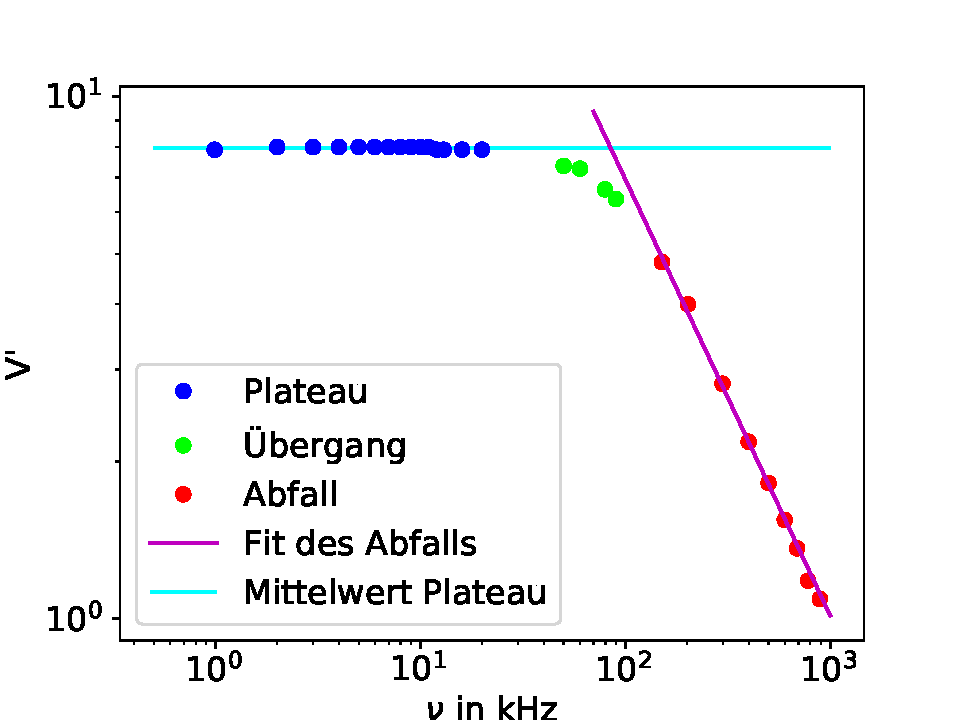
\includegraphics[width=\textwidth]{verhaeltnis1.pdf}%[trim = 5mm 3mm 5mm 5mm, clip, width=\textwidth]{verhaeltnis1.pdf}
                        \caption{Widerstandsverhältnis 10.}
                        \label{fig:pep2}
                    \end{subfigure}
                    \begin{subfigure}{0.48\textwidth}
                        \centering
                        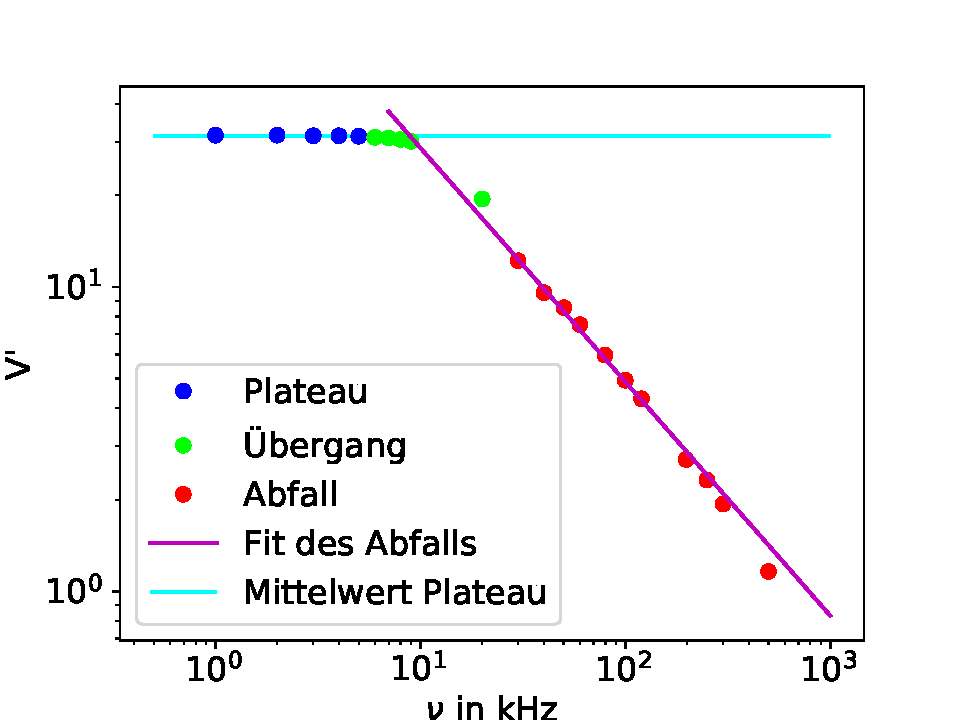
\includegraphics[width=\textwidth]{verhaeltnis2.pdf}%[trim = 5mm 3mm 5mm 5mm, clip, width=\textwidth]{verhaeltnis2.pdf}
                        \caption{Widerstandsverhältnis 33,1.}
                        \label{fig:TU}
                    \end{subfigure}
                    \begin{subfigure}{0.48\textwidth}
                        \centering
                        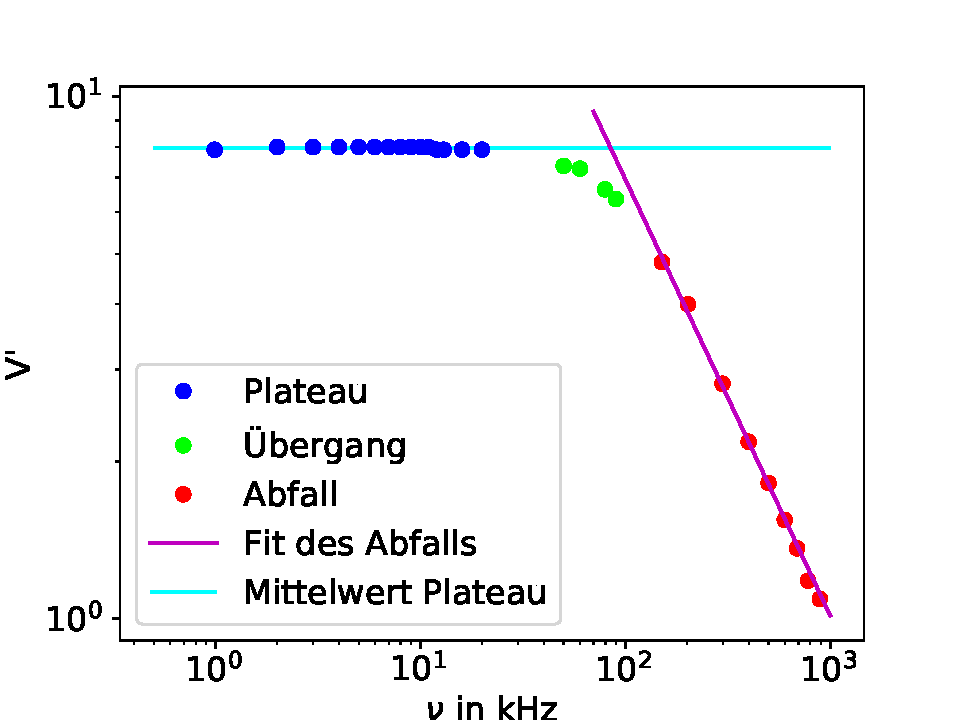
\includegraphics[width=\textwidth]{verhaeltnis1.pdf}%[trim = 0mm 3mm 5mm 5mm, clip, width=\textwidth]{verhaeltnis3.pdf}
                        \caption{Widerstandsverhältnis 3,31.}
                        \label{fig:TU}
                    \end{subfigure}
                    \begin{subfigure}{0.48\textwidth}
                        \centering
                        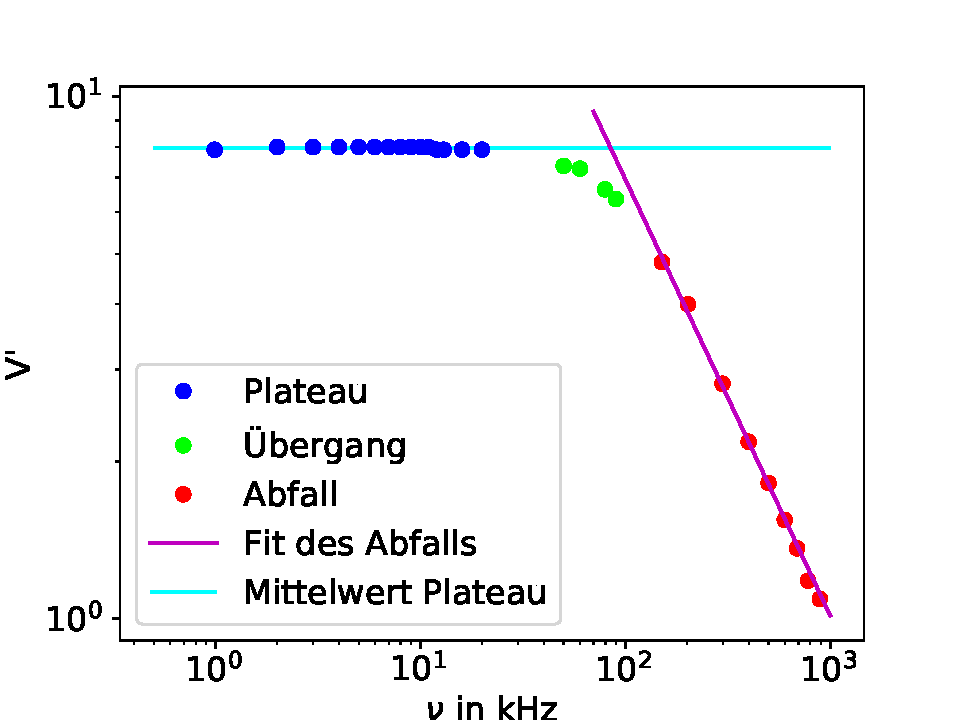
\includegraphics[width=\textwidth]{verhaeltnis1.pdf}%[trim = 0mm 3mm 5mm 5mm, clip, width=\textwidth]{verhaeltnis4.pdf}
                        \caption{Widerstandsverhältnis 2,96.}
                        \label{fig:TU}
                    \end{subfigure}
                    \caption{Zusammenhang zwischen Frequenz und Verstärkung für verschiedene Widerstandsverhältnisse.}
                    \label{fig:plateaus}
                \end{figure}


                Aus diesen Fitparametern und dem Plateau $P$ kann nun die Grenzfrequenz 

                \begin{align*}
                    \nu_{Grenz} = \left(\frac{P}{\sqrt{2}a}\right)^{\frac1b},
                \end{align*}

                die Leerlaufverstärkung 

                \begin{align*}
                    V = \frac{P\cdot R_N}{R_N+R_1\cdot P}
                \end{align*}

                und das Bandbreitenprodukt

                \begin{align*}
                    B = V'\cdot \nu_{Grenz}
                \end{align*}

                errechnet werden. Für die vier Messreihen sind die Werte in Tabelle \ref{tab:grenz} angegeben.


                \begin{table}
                    \centering
                    \caption{Grenzfrequenz, Leerlaufverstärkung und Bandbreitenprodukt für die jeweiligen Widerstandsverhältnisse
                    des invertierenden Linearverstärkers.}
                    \label{tab:grenz}
                    \begin{tabular}{c c c c c}
                        \toprule
                            Widerstandsverhältnis & $\nu_{Grenz}$/kHz & $V$ & $B$/kHz\\
                        \midrule
                            10   & $ 128,38 $ & $  4,44 $ & $ 1023 $ \\
                            33,1 & $  13,92 $ & $ 16,11 $ & $  437 $ \\
                            3,31 & $ 204,16 $ & $  0,28 $ & $  744 $ \\
                            2,96 & $ 238,01 $ & $  0,31 $ & $  791 $ \\
                        \bottomrule
                    \end{tabular}
                \end{table}

            \subsubsection{Frequenzabhängigkeit der Phase zwischen Ein- und Ausgangsspannung}


                Für die vier Messreihen wird die Abhängigkeit der Phase zwischen Ein- und Ausgangsspannung
                von der Frequenz in Abb. \ref{fig:phase} graphisch dargestellt. Dabei fällt der Phasenunterschied
                mit steigender Frequenz von 180° auf Werte zwischen und 40 und 100° ab. Dieses Verhalten erinnert 
                an einen Tiefpass.

                \begin{figure}[H]
                    \centering
                    \begin{subfigure}{0.48\textwidth}
                        \centering
                        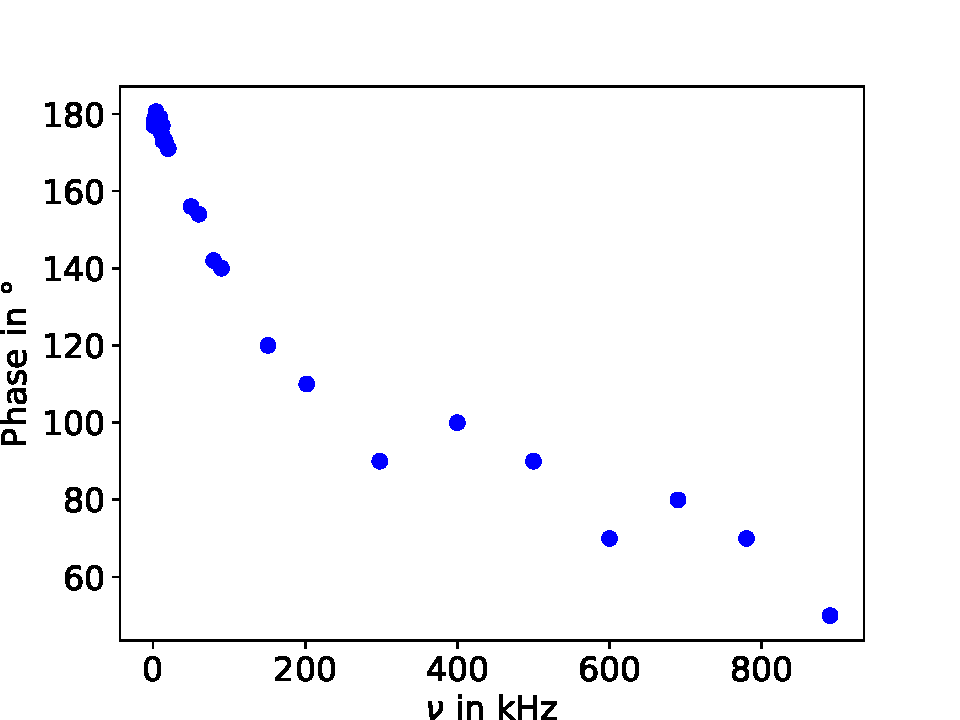
\includegraphics[width=\textwidth]{phase1.pdf}%[trim = 5mm 3mm 5mm 5mm, clip, width=\textwidth]{phase1.pdf}
                        \caption{Widerstandsverhältnis 10.}
                        \label{fig:pep2}
                    \end{subfigure}
                    \begin{subfigure}{0.48\textwidth}
                        \centering
                        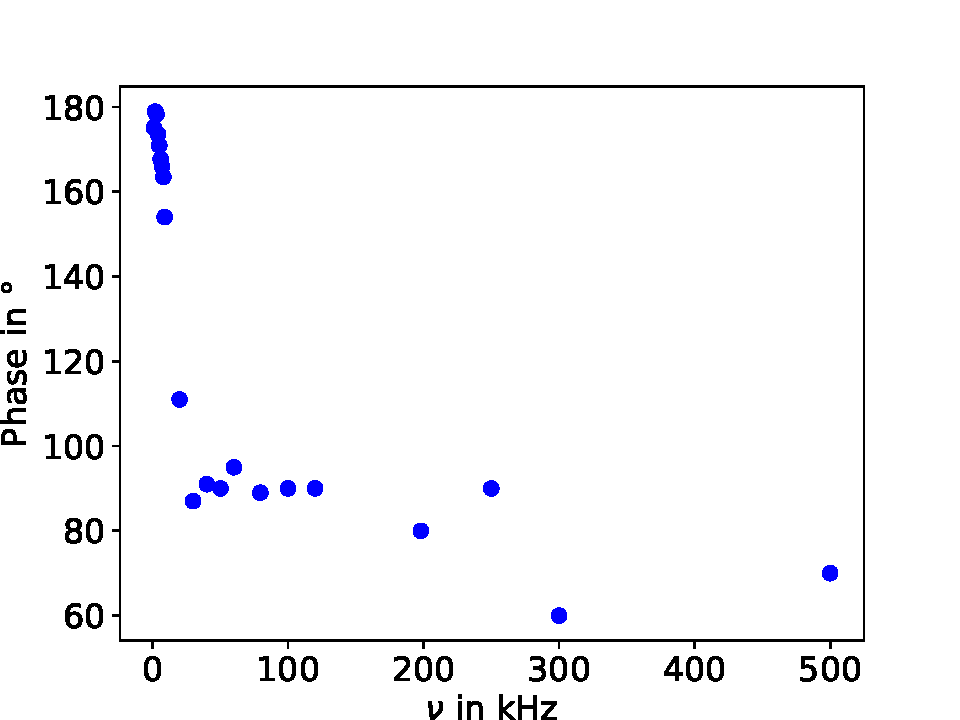
\includegraphics[width=\textwidth]{phase2.pdf}%[trim = 5mm 3mm 5mm 5mm, clip, width=\textwidth]{phase2.pdf}
                        \caption{Widerstandsverhältnis 33,1.}
                        \label{fig:TU}
                    \end{subfigure}
                    \begin{subfigure}{0.48\textwidth}
                        \centering
                        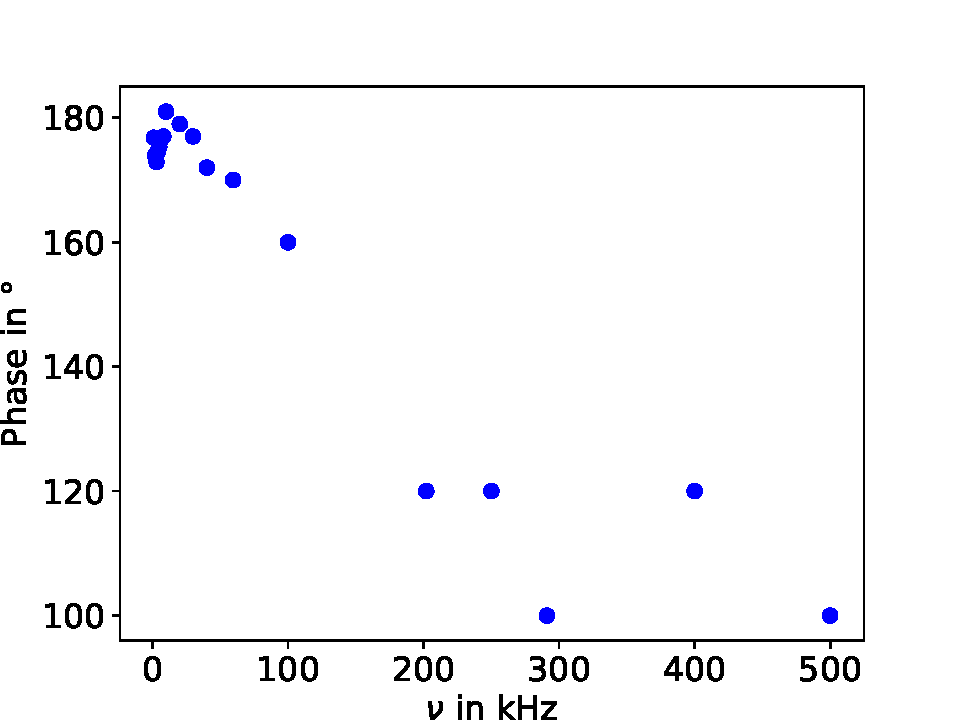
\includegraphics[width=\textwidth]{phase3.pdf}%[trim = 0mm 3mm 5mm 5mm, clip, width=\textwidth]{phase3.pdf}
                        \caption{Widerstandsverhältnis 3,31.}
                        \label{fig:TU}
                    \end{subfigure}
                    \begin{subfigure}{0.48\textwidth}
                        \centering
                        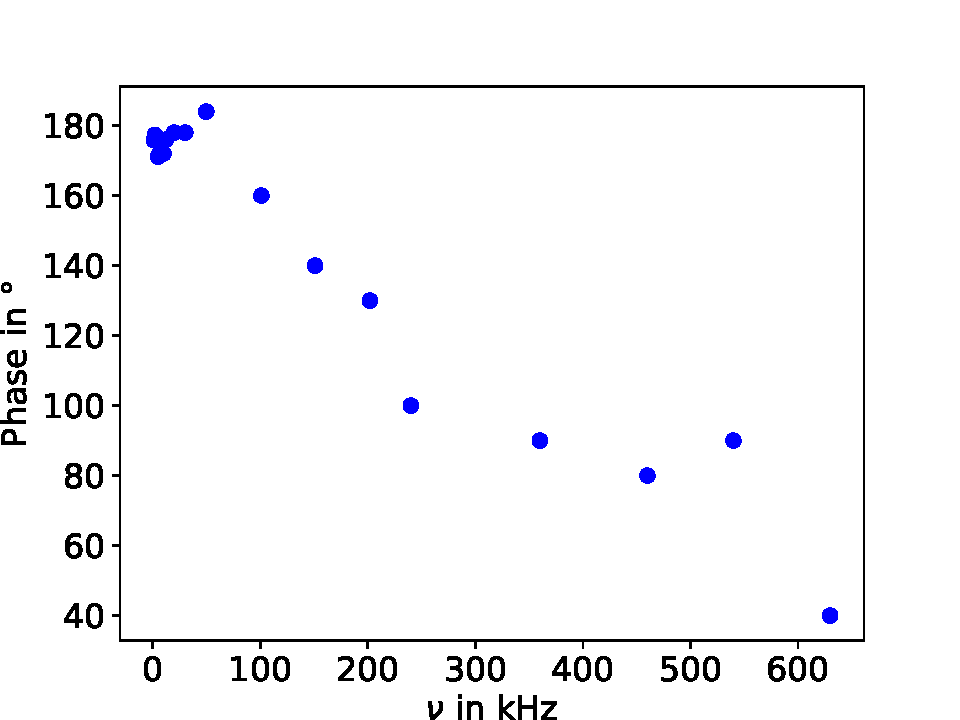
\includegraphics[width=\textwidth]{phase4.pdf}%[trim = 0mm 3mm 5mm 5mm, clip, width=\textwidth]{phase4.pdf}
                        \caption{Widerstandsverhältnis 2,96.}
                        \label{fig:TU}
                    \end{subfigure}
                    \caption{Frequenzabhängigkeit der Phase für verschiedene Widerstandsverhältnisse beim invertierenden Linearverstärker.}
                    \label{fig:phase}
                \end{figure}

        \subsection{Umkehrintegrator}

            In Abb. \ref{fig:int} sind die Werte für Ausgangsspannung in einem doppelt logarithmischen Diagramm 
            gegen die Frequenz aufgetragen. Sie werden in einem ausgewählten Bereich mit einer Potenzfunktion gefittet, 
            deren Parameter sich zu 

            \begin{align*}
                a &= (60,3\pm 0,5)\,\symup{V} \\
                b &= (-0,923\pm 0,003)\,\frac{\symup{V}}{\symup{kHz}} \\
            \end{align*}

            ergeben. Der Fit bestätigt, dass beim Integrator die Ausgangsspannung mit der Frequenz abnimmt.

            \begin{figure}
                \centering
                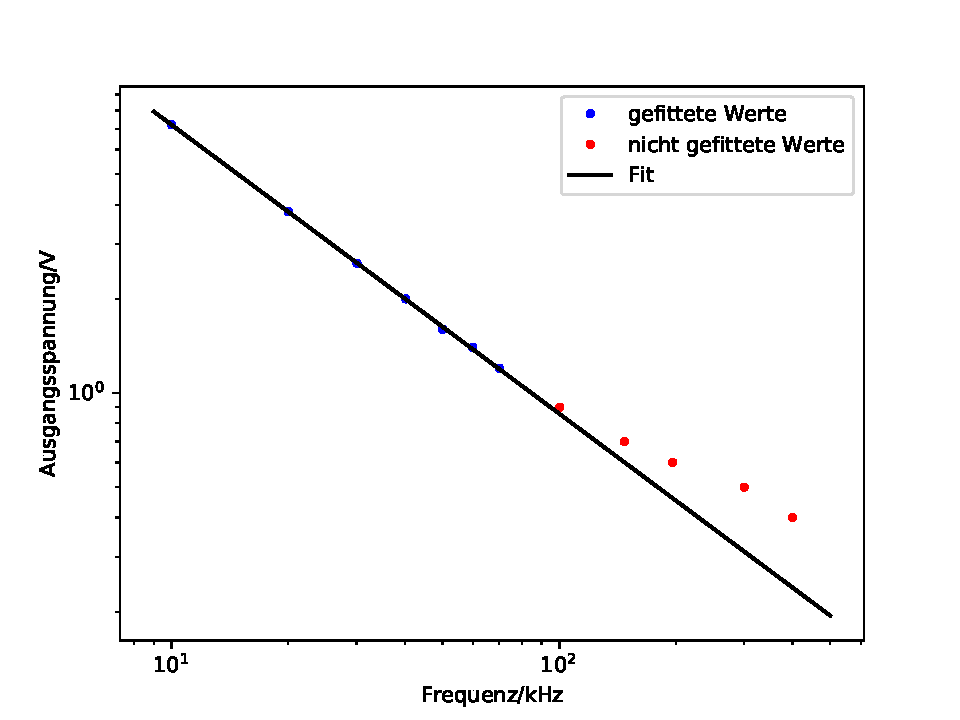
\includegraphics[height=8cm]{integrator.pdf}
                \caption{Ausgangsspannung in Abhängigkeit von der Frequenz 
                beim Umkehrintegrator mit R = 33,1\,k$\symup{\Omega}$ und C = 0,015\,nF.}
                \label{fig:int}
            \end{figure}

            Beispielhaft sind in Abb. \ref{fig:dreiint} drei Ausgangsspannungen (grün)
            mit ihren jeweiligen integrierten Spannungen (gelb) zu sehen. Es wird deutlich dass dabei 
            eine Sinusspannung zu einem Cosinus, eine Dreiecksspannung zu einem Sinus und eine 
            Rechteckspannung zu einer Dreiecksspannung wird.

                \begin{figure}
                    \centering
                    \begin{subfigure}{0.48\textwidth}
                        \centering
                        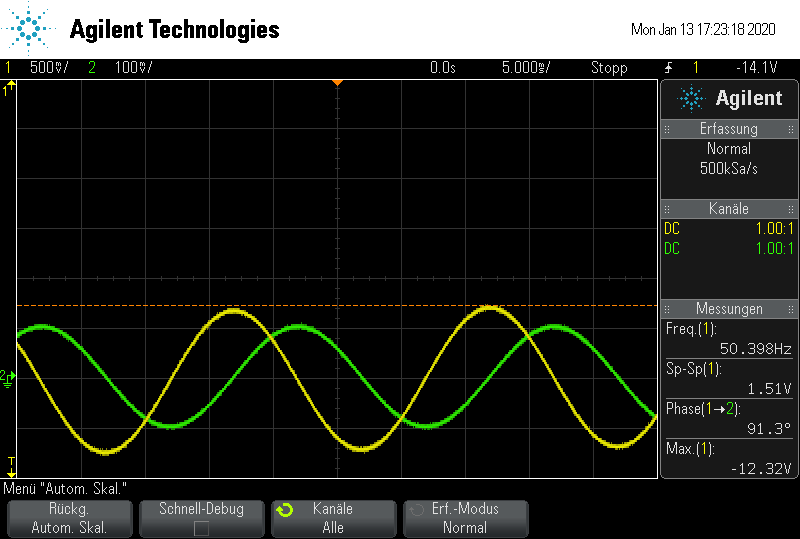
\includegraphics[width=\textwidth]{scope_5.png}%[trim = 0mm 20mm 45mm 20mm, clip, width=\textwidth]{scope_5.png}
                        \caption{Sinus und Integration (Cosinus).}
                        \label{fig:TU}
                    \end{subfigure}
                    \begin{subfigure}{0.48\textwidth}
                        \centering
                        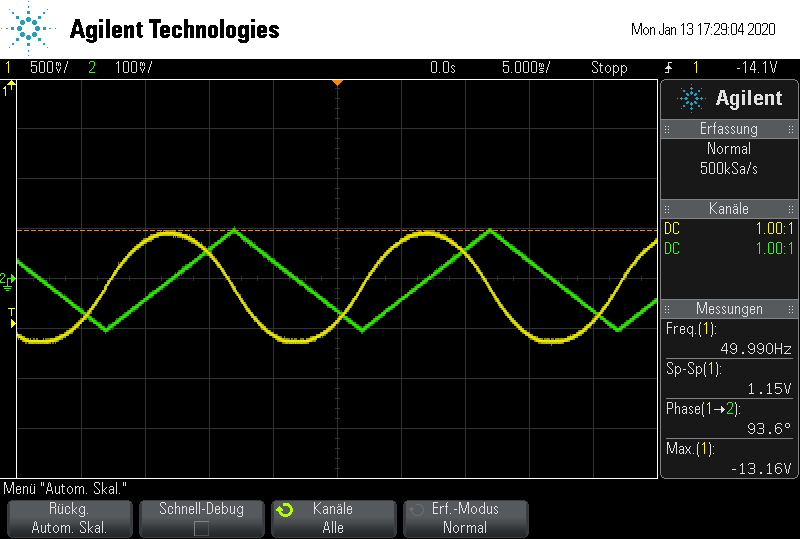
\includegraphics[width=\textwidth]{scope_7.png}%[trim = 0mm 20mm 45mm 20mm, clip, width=\textwidth]{scope_7.png}
                        \caption{Dreieck und Integration (Sinus).}
                        \label{fig:TU}
                    \end{subfigure}
                    \begin{subfigure}{0.48\textwidth}
                        \centering
                        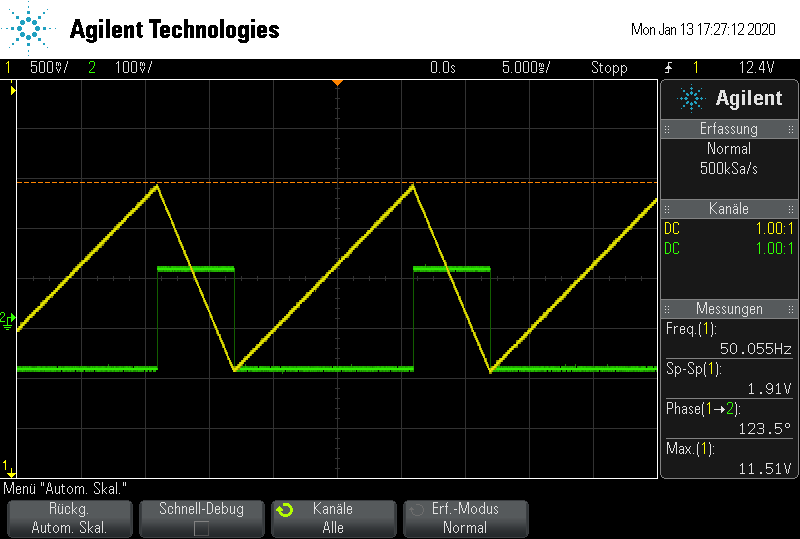
\includegraphics[width=\textwidth]{scope_6.png}%[trim = 0mm 20mm 45mm 20mm, clip, width=\textwidth]{scope_6.png}
                        \caption{Rechteck und Integration (Dreieck).}
                        \label{fig:TU}
                    \end{subfigure}
                    \caption{Verschiedene Ausgangsspannungen (grün) mit jeweiliger Integration (gelb) für den Umkehrintegrator.}
                    \label{fig:dreiint}
                \end{figure}



        \subsection{Differenzierer}

            Für den Differenzierer wird ebenfalls die Ausgangsspannung doppelt logarithmisch gegen die Frequenz 
            geplottet (Abb. \ref{fig:diff}).

            \begin{figure}
                \centering
                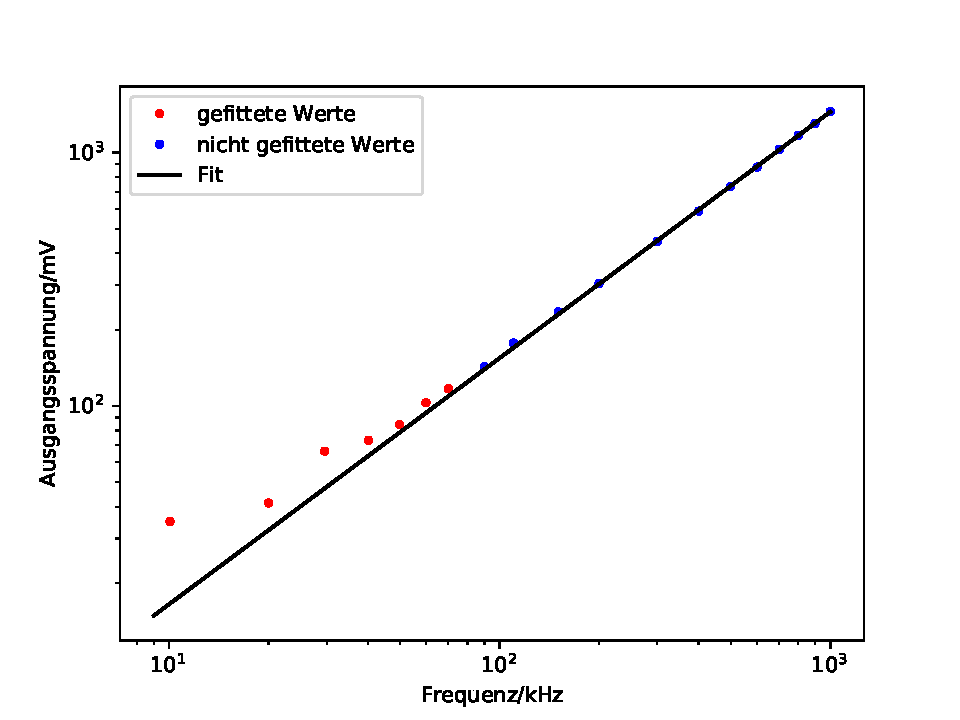
\includegraphics[height=8cm]{differenzierer.pdf}
                \caption{Ausgangsspannung in Abhängigkeit von der Frequenz 
                beim Differenzierer mit R = 33,1\,k$\symup{\Omega}$ und C = 0,015\,nF.}
                \label{fig:diff}
            \end{figure}

            Die im ausgewählten Bereich aus dem Fit ermittelten Parameter sind

            \begin{align*}
                a &= (1,76\pm 0,05)\,\symup{mV}\\
                b &= (0,972\pm 0,005)\,\frac{\symup{mV}}{\symup{kHz}}.\\
            \end{align*}

            Hier bestätigt sich der Anstieg der Ausgangsspannung mit wachsender Frequenz für den Differenzierer.
            Die drei Spannungsformen Sinus, Rechteck und Dreieck werden durch den Differenzierer geleitet und mit 
            den jeweiligen Ausgangsspannungen in Form von Cosinus, Delta-Peaks und Rechteckspannung dargestellt (siehe Abb. 
            \ref{fig:dreidiff}).

                \begin{figure}
                    \centering
                    \begin{subfigure}{0.48\textwidth}
                        \centering
                        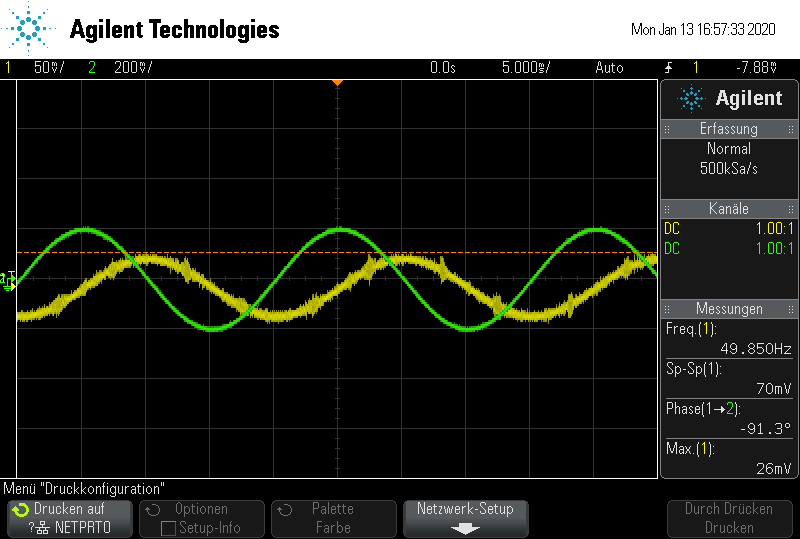
\includegraphics[width=\textwidth]{scope_0.png}%[trim = 0mm 20mm 45mm 20mm, clip, width=\textwidth]{scope_0.png}
                        \caption{Sinus und Ableitung (Cosinus).}
                        \label{fig:TU}
                    \end{subfigure}
                    \begin{subfigure}{0.48\textwidth}
                        \centering
                        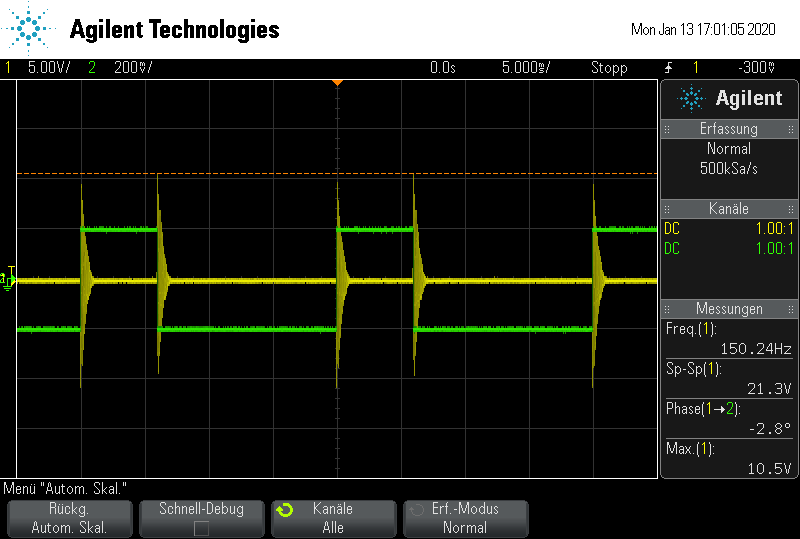
\includegraphics[width=\textwidth]{scope_2.png}%[trim = 0mm 20mm 45mm 20mm, clip, width=\textwidth]{scope_2.png}
                        \caption{Rechteck und Ableitung (Delta-Peaks).}
                        \label{fig:TU}
                    \end{subfigure}
                    \begin{subfigure}{0.48\textwidth}
                        \centering
                        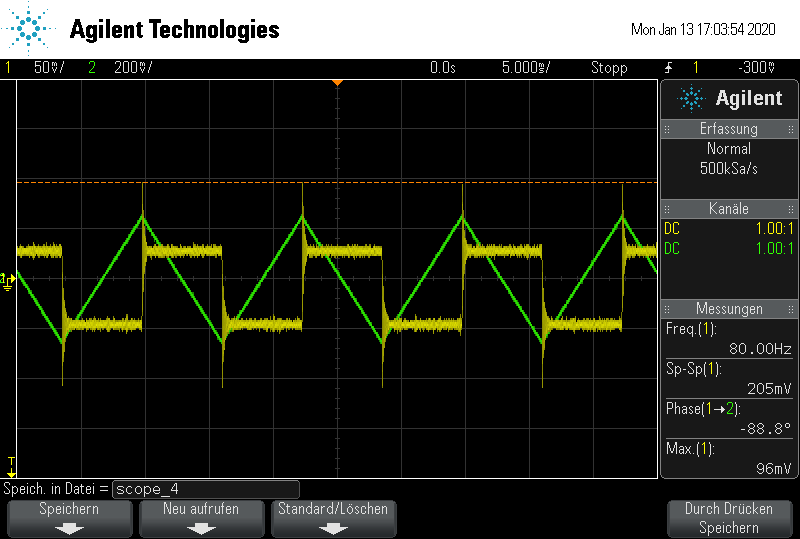
\includegraphics[width=\textwidth]{scope_4.png}%[trim = 0mm 20mm 45mm 20mm, clip, width=\textwidth]{scope_4.png}
                        \caption{Dreieck und Ableitung (Rechteck).}
                        \label{fig:TU}
                    \end{subfigure}
                    \caption{Verschiedene Eingangsspannungen (grün) mit jeweiliger Ableitung (gelb) für den Differenzierer.}
                    \label{fig:dreidiff}
                \end{figure}


        \subsection{Nicht-Invertierender Schmitt-Trigger}

            In Abbildung \ref{fig:schmitt} ist das sinusförmige Eingangssignal sowie 
            das Ausgangssignal der nicht-invertierenden Schmitt-Trigger-Schaltung zu sehen.
            Daraus kann eine Schalthysterese von 160\,mV abgelesen werden.

            \begin{figure}[H]
                \centering 
                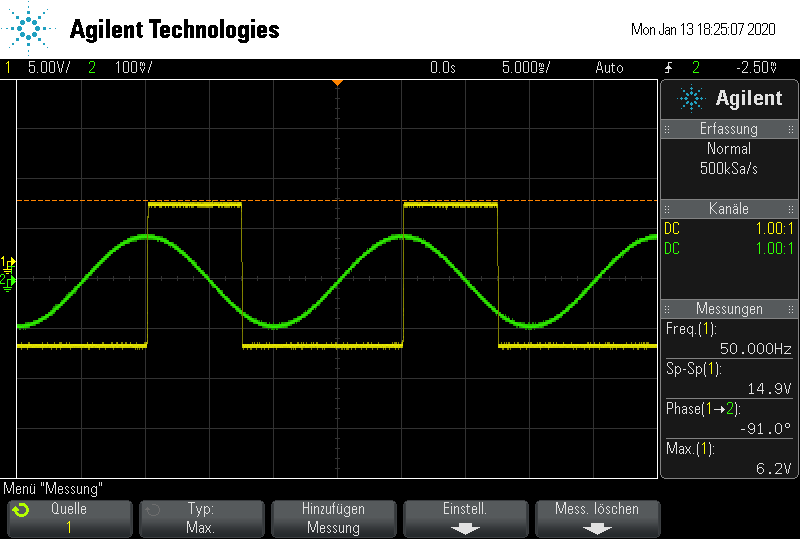
\includegraphics[height=5cm]{scope_9.png}
                \caption{Abbildung des Scheitelwerts des nicht-invertierenden Schmitt-Triggers, wobei die 
                Eingangsspannung grün und die Ausgangsspannung gelb ist.}
                \label{fig:schmitt}
            \end{figure}

            Wenn die Schalthysterese mithilfe der Formel

            \begin{align*}
                U_{\symup{{Hys}}} = 2\frac{R_1}{R_2}U_B
            \end{align*}

            berechnet wird, ergibt sich eine Schalthysterese von 3\,V für die 
            notierten Parameter $R_1=10\,$k$\symup{\Omega}$, $R_2=100\,$k$\symup{\Omega}$ und $U_B=15$\,V.
            Diese ist viel größer als die tatsächlich gemessene (160\,mV), weshalb davon auszugehen ist,
            dass die Größenordnung eines Parameters falsch notiert wurde.


        \subsection{Signalgenerator}

            Das mit dem Signalgenerator erzeugte Signal sowie das sinusförmige Eingangssignal 
            sind in Abb. \ref{fig:schmittint} zu erkennen. Die Amplitude des Dreieckssignals 
            kann zu 95,5\,mV abgelesen werden. Die Frequenz liegt bei 1,757\,kHz.

            \begin{figure}[H]
                \centering 
                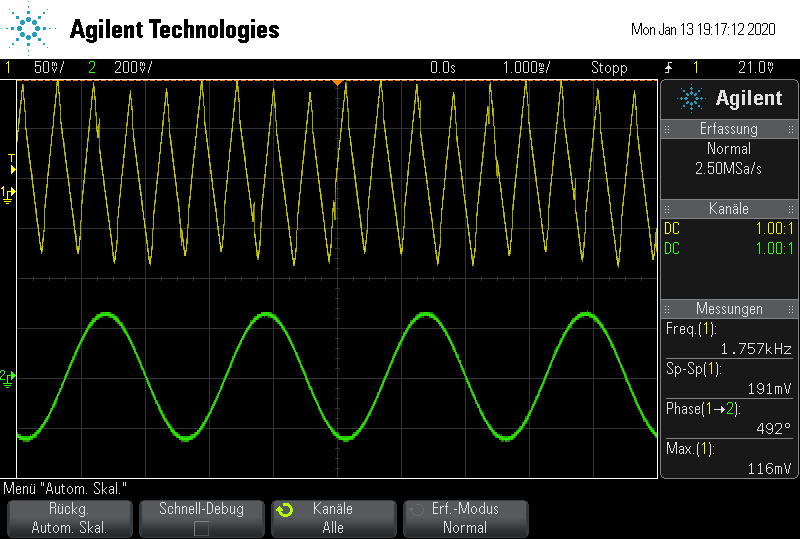
\includegraphics[height=5cm]{scope_11.png}
                \caption{Abbildung des Eingangssignals (grün) und Ausgangssignals (gelb) des Signalgenerators.}
                \label{fig:schmittint}
            \end{figure}

            Die theoretische Frequenz lässt sich über 

            \begin{align*}
                \nu_{theo} = \frac{R_2}{4CR_1R_3} 
            \end{align*}

            zu 1,025\,kHz berechnen, wobei die Werte $R_1=R_3=10$\,k$\symup{\Omega}$, $R_2=100$\,k$\symup{\Omega}$
            und $C=975$\,nF einegesetzt werden.

            

        \subsection{Variierende Amplituden}

            Die Bilder, die für die Schaltung mit variierenden Amplituden aufgenommen werden, 
            sind in Abb. \ref{fig:vari} zu sehen. Es ist zu erkennen, dass die eintreffende 
            reine Rechteckspannung in eine Rechteckspannung mit Oszillationen umgewandelt wird. 
            

            \begin{figure}[H]
                \centering
                \begin{subfigure}{0.48\textwidth}
                        \centering
                        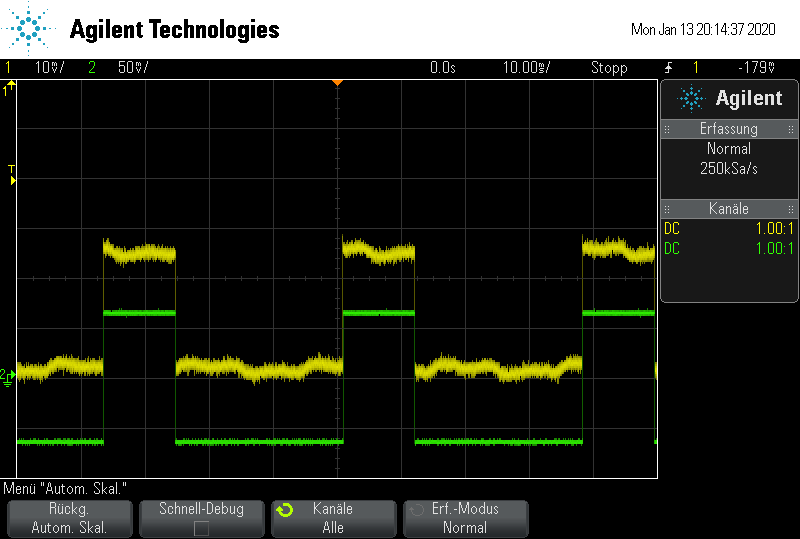
\includegraphics[width=\textwidth]{scope_13.png}%[trim = 0mm 20mm 45mm 20mm, clip, width=\textwidth]{scope_13.png}
                        %\caption{Sinus und Ableitung.}
                        \label{fig:TU}
                    \end{subfigure}
                    \begin{subfigure}{0.48\textwidth}
                        \centering
                        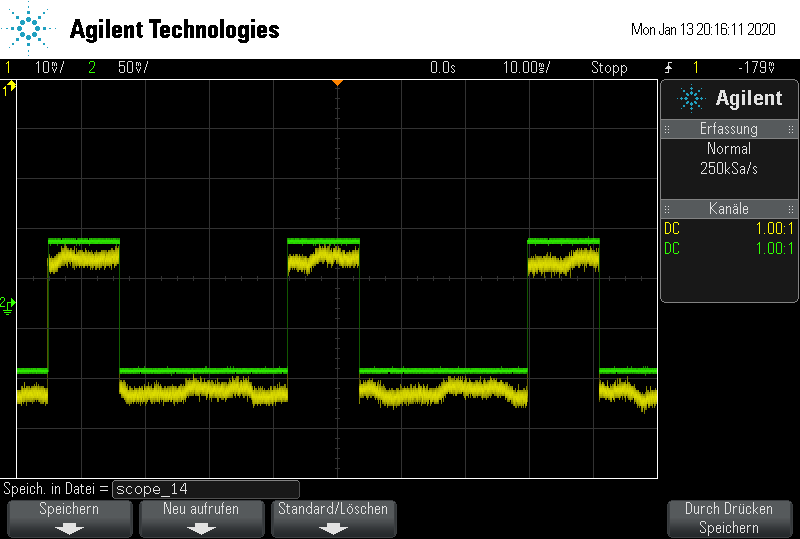
\includegraphics[width=\textwidth]{scope_14.png}%[trim = 0mm 20mm 45mm 20mm, clip, width=\textwidth]{scope_14.png}
                        %\caption{Rechteck und Ableitung.}
                        \label{fig:TU}
                    \end{subfigure}
                    \begin{subfigure}{0.48\textwidth}
                        \centering
                        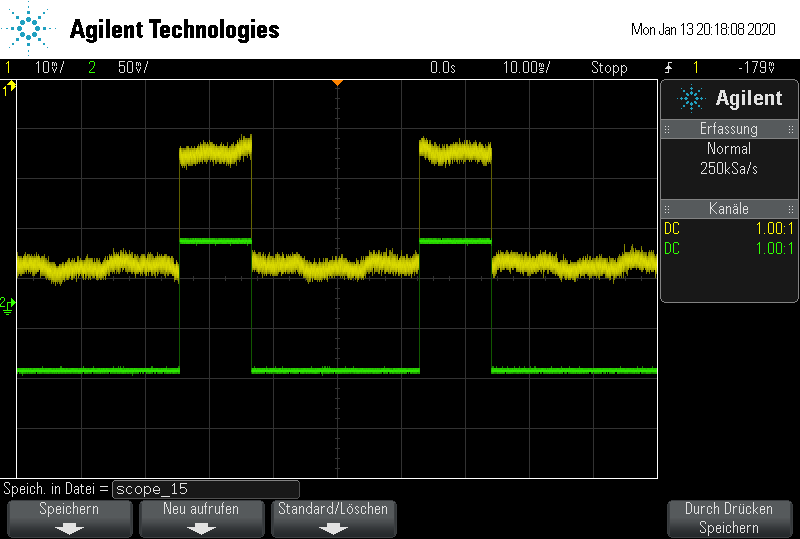
\includegraphics[width=\textwidth]{scope_15.png}%[trim = 0mm 20mm 45mm 20mm, clip, width=\textwidth]{scope_15.png}
                        %\caption{Dreieck und Ableitung.}
                        \label{fig:TU}
                    \end{subfigure}
                \caption{Aufgenommene Bilder zur Schaltung der variierenden Amplituden.}
                \label{fig:vari}
            \end{figure}

            Allerdings sollte die Schaltung bei richtiger Funktionsweise keine Rechteckspannung mit Oszillationsanteil,
            sondern eine reine gedämpfte oder verstäkrte Sinusspannung ausgeben. Da dies nicht der Fall ist, ist vermutlich 
            eines der Bauteile falsch eingebaut worden.
